%-----------------------------------
% Define document and include general packages
%-----------------------------------
% Tabellen- und Abkürzungsverzeichnis stehen normalerweise nicht im
% Inhaltsverzeichnis. Gleiches gilt für das Abkürzungsverzeichnis (siehe unten).
% Manche Dozenten bemängeln das. Die Optionen 'listof=totoc,bibliography=totoc'
% geben das Tabellen- und Abkürzungsverzeichnis im Inhaltsverzeichnis (toc=Table
% of Content) aus.
% Da es aber verschiedene Regelungen je nach Dozent geben kann, werden hier
% beide Varianten dargestellt.
%\documentclass[12pt,oneside,titlepage,listof=totoc,bibliography=totoc]{scrartcl}
\documentclass[12pt,oneside,titlepage]{scrartcl}
%Dokumentensprache
\newif\ifde
\newif\ifen

%-----------------------------------
% Meta informationen
%-----------------------------------
%-----------------------------------
% Meta Informationen zur Arbeit
%-----------------------------------

% Autor
\newcommand{\myAutor}{Mohamadreza Sabaghian}

% Adresse
\newcommand{\myAdresse}{Am Mitterfeld 27 \\ \> \> \> 81829 München}

% Titel der Arbeit
\newcommand{\myTitel}{Modeling the Effect of Fiscal and Monetary Policy on Housing Price} 
\newcommand{\mySubtitel}{in Germany between Years 2000 and 2020} 


% Matrikelnummer
\newcommand{\myMatrikelNr}{556076}

% Ort
\newcommand{\myOrt}{München}

% Datum der Abgabe
\newcommand{\myAbgabeDatum}{\today}


% Studiengang
\newcommand{\myStudiengang}{Master of Business Administration (MBA)}



% Assignment
\newcommand{\myAssignment}{No. 1}

% Instructor
\newcommand{\myInstructor}{Prof. Dr. Gerald Mann}

% Semester
\newcommand{\mySemester}{1st Academic Semester 2020}

% Module
\newcommand{\myModule}{Economics}

%Englisch
\entrue
\usepackage[english]{babel}





\newcommand{\langde}[1]{%
   \ifde\selectlanguage{ngerman}#1\fi}
\newcommand{\langen}[1]{%
   \ifen\selectlanguage{english}#1\fi}
\langde{\usepackage[babel,german=quotes]{csquotes}}
\langen{\usepackage[babel,english=british]{csquotes}}
\usepackage[utf8]{luainputenc}
\usepackage[T1]{fontenc}
\usepackage{fancyhdr}
\usepackage{fancybox}
\usepackage[a4paper, left=4cm, right=2cm, top=4cm, bottom=2cm]{geometry}
\usepackage{graphicx}
\usepackage{colortbl}
\usepackage[capposition=top]{floatrow}
\usepackage{array}
\usepackage{float}      %Positionierung von Abb. und Tabellen mit [H] erzwingen
\usepackage{footnote}
% Darstellung der Beschriftung von Tabellen und Abbildungen (Leitfaden S. 44)
% singlelinecheck=false: macht die Caption linksbündig (statt zentriert)
% labelfont auf fett: (Tabelle x.y:, Abbildung: x.y)
% font auf fett: eigentliche Bezeichnung der Abbildung oder Tabelle
% Fettschrift laut Leitfaden 2018 S. 45
\usepackage[singlelinecheck=false, labelfont=bf, font=bf]{caption}
\usepackage{caption}
\usepackage{enumitem}
\usepackage{amssymb}
\usepackage{mathptmx}
%\usepackage{minted} %Kann für schöneres Syntax Highlighting genutzt werden. ACHTUNG: Python muss installiert sein.
\usepackage[scaled=0.9]{helvet} % Behebt, zusammen mit Package courier, pixelige Überschriften. Ist, zusammen mit mathptx, dem times-Package vorzuziehen. Details: https://latex-kurs.de/fragen/schriftarten/Times_New_Roman.html
\usepackage{courier}
\usepackage{amsmath}
\usepackage[table]{xcolor}
\usepackage{marvosym}			% Verwendung von Symbolen, z.B. perfektes Eurozeichen
\usepackage[colorlinks=true,linkcolor=black]{hyperref}
\definecolor{darkblack}{rgb}{0,0,0}
\hypersetup{colorlinks=true, breaklinks=true, linkcolor=darkblack, menucolor=darkblack, urlcolor=darkblack}
\renewcommand\familydefault{\sfdefault}
\usepackage{ragged2e}

% Mehrere Fussnoten nacheinander mit Komma separiert
\usepackage[hang, multiple]{footmisc}
\setlength{\footnotemargin}{1em}

% todo Aufgaben als Kommentare verfassen für verschiedene Editoren
\usepackage{todonotes}

%Pakete für Tabellen
\usepackage{epstopdf}
\usepackage{nicefrac} % Brüche
\usepackage{multirow}
\usepackage{rotating} % vertikal schreiben
\usepackage{mdwlist}
\usepackage{tabularx}% für breitenangabe

\definecolor{dunkelgrau}{rgb}{0.8,0.8,0.8}
\definecolor{hellgrau}{rgb}{0.0,0.7,0.99}
% Colors for listings
\definecolor{mauve}{rgb}{0.58,0,0.82}
\definecolor{dkgreen}{rgb}{0,0.6,0}

% sauber formatierter Quelltext
\usepackage{listings}
% JavaScript als Sprache definieren:
\lstdefinelanguage{JavaScript}{
	keywords={break, super, case, extends, switch, catch, finally, for, const, function, try, continue, if, typeof, debugger, var, default, in, void, delete, instanceof, while, do, new, with, else, return, yield, enum, let, await},
	keywordstyle=\color{blue}\bfseries,
	ndkeywords={class, export, boolean, throw, implements, import, this, interface, package, private, protected, public, static},
	ndkeywordstyle=\color{darkgray}\bfseries,
	identifierstyle=\color{black},
	sensitive=false,
	comment=[l]{//},
	morecomment=[s]{/*}{*/},
	commentstyle=\color{purple}\ttfamily,
	stringstyle=\color{red}\ttfamily,
	morestring=[b]',
	morestring=[b]"
}

\lstset{
	%language=JavaScript,
	numbers=left,
	numberstyle=\tiny,
	numbersep=5pt,
	breaklines=true,
	showstringspaces=false,
	frame=l ,
	xleftmargin=5pt,
	xrightmargin=5pt,
	basicstyle=\ttfamily\scriptsize,
	stepnumber=1,
	keywordstyle=\color{blue},          % keyword style
  	commentstyle=\color{dkgreen},       % comment style
  	stringstyle=\color{mauve}         % string literal style
}

% Biblatex

%%%% Neuer Leitfaden (2018)
\usepackage[ 
backend=biber,
style=ext-authoryear,
maxcitenames=3,	% mindestens 3 Namen ausgeben bevor et. al. kommt
maxbibnames=999,
mergedate=false,
date=iso,
seconds=true, %werden nicht verwendet, so werden aber Warnungen unterdrückt.
urldate=iso,
innamebeforetitle,
dashed=false,
autocite=footnote,
doi=false,
useprefix=true, % 'von' im Namen beachten (beim Anzeigen)
mincrossrefs = 1
]{biblatex}%iso dateformat für YYYY-MM-DD

%weitere Anpassungen für BibLaTex
\input{skripte/modsBiblatex2018}

%%%%% Alter Leitfaden. Ggf. Einkommentieren und Bereich hierüber auskommentieren
%\usepackage[
%backend=biber,
%style=numeric,
%citestyle=authoryear,
%url=false,
%isbn=false,
%notetype=footonly,
%hyperref=false,
%sortlocale=de]{biblatex}

%weitere Anpassungen für BibLaTex
%\input{skripte/modsBiblatex}

%%%% Ende Alter Leitfaden

%Bib-Datei einbinden
\addbibresource{literatur/literatur.bib}

% Zeilenabstand im Literaturverzeichnis ist Einzeilig
% siehe Leitfaden S. 14
\AtBeginBibliography{\singlespacing}

%Silbentrennung
\usepackage{hyphsubst}
\HyphSubstIfExists{ngerman-x-latest}{%
\HyphSubstLet{ngerman}{ngerman-x-latest}}{}

% Pfad fuer Abbildungen
\graphicspath{{./}{./abbildungen/}}

%-----------------------------------
% Weitere Ebene einfügen
%-----------------------------------
\input{skripte/weitereEbene}

%-----------------------------------
% Paket für die Nutzung von Anhängen
%-----------------------------------
\usepackage{appendix}

 
%-----------------------------------
% Zeilenabstand 1,5-zeilig
%-----------------------------------
\usepackage{setspace}
\onehalfspacing

%-----------------------------------
% Absätze durch eine neue Zeile
%-----------------------------------
\setlength{\parindent}{0mm}
\setlength{\parskip}{0.8em plus 0.5em minus 0.3em}

\sloppy					%Abstände variieren
\pagestyle{headings}

%-----------------------------------
% Abkürzungsverzeichnis
%-----------------------------------
\usepackage[printonlyused]{acronym}

%-----------------------------------
% PDF Meta Daten setzen
%-----------------------------------
\hypersetup{
    pdfinfo={
        Title={\myTitel},
        Subject={\myStudiengang},
        Author={\myAutor},
        Build=1.1
    }
}

%-----------------------------------
% Umlaute in Code korrekt darstellen
% siehe auch: https://en.wikibooks.org/wiki/LaTeX/Source_Code_Listings
%-----------------------------------
\lstset{literate=
	{á}{{\'a}}1 {é}{{\'e}}1 {í}{{\'i}}1 {ó}{{\'o}}1 {ú}{{\'u}}1
	{Á}{{\'A}}1 {É}{{\'E}}1 {Í}{{\'I}}1 {Ó}{{\'O}}1 {Ú}{{\'U}}1
	{à}{{\`a}}1 {è}{{\`e}}1 {ì}{{\`i}}1 {ò}{{\`o}}1 {ù}{{\`u}}1
	{À}{{\`A}}1 {È}{{\'E}}1 {Ì}{{\`I}}1 {Ò}{{\`O}}1 {Ù}{{\`U}}1
	{ä}{{\"a}}1 {ë}{{\"e}}1 {ï}{{\"i}}1 {ö}{{\"o}}1 {ü}{{\"u}}1
	{Ä}{{\"A}}1 {Ë}{{\"E}}1 {Ï}{{\"I}}1 {Ö}{{\"O}}1 {Ü}{{\"U}}1
	{â}{{\^a}}1 {ê}{{\^e}}1 {î}{{\^i}}1 {ô}{{\^o}}1 {û}{{\^u}}1
	{Â}{{\^A}}1 {Ê}{{\^E}}1 {Î}{{\^I}}1 {Ô}{{\^O}}1 {Û}{{\^U}}1
	{œ}{{\oe}}1 {Œ}{{\OE}}1 {æ}{{\ae}}1 {Æ}{{\AE}}1 {ß}{{\ss}}1
	{ű}{{\H{u}}}1 {Ű}{{\H{U}}}1 {ő}{{\H{o}}}1 {Ő}{{\H{O}}}1
	{ç}{{\c c}}1 {Ç}{{\c C}}1 {ø}{{\o}}1 {å}{{\r a}}1 {Å}{{\r A}}1
	{€}{{\EUR}}1 {£}{{\pounds}}1 {„}{{\glqq{}}}1
}

%-----------------------------------
% Kopfbereich / Header definieren
%-----------------------------------
\pagestyle{fancy}
\fancyhf{}
% Seitenzahl oben, mittig, mit Strichen beidseits
% \fancyhead[C]{-\ \thepage\ -}

% Seitenzahl oben, mittig, entsprechend Leitfaden ohne Striche beidseits
\fancyhead[C]{\thepage}
%\fancyhead[L]{\leftmark}							% kein Footer vorhanden
% Waagerechte Linie unterhalb des Kopfbereiches anzeigen. Laut Leitfaden ist
% diese Linie nicht erforderlich. Ihre Breite kann daher auf 0pt gesetzt werden.
\renewcommand{\headrulewidth}{0.4pt}
%\renewcommand{\headrulewidth}{0pt}


%-----------------------------------
% Start the document here:
%-----------------------------------
\begin{document}

\pagenumbering{Roman}								% Seitennumerierung auf römisch umstellen
\renewcommand{\refname}{\langde{Literaturverzeichnis}
						\langen{Bibliography}}		% "Literatur" in
%"Literaturverzeichnis" umbenennen
\newcolumntype{C}{>{\centering\arraybackslash}X}	% Neuer Tabellen-Spalten-Typ:
%Zentriert und umbrechbar

%-----------------------------------
% Titlepage
%-----------------------------------
\begin{titlepage}
	\newgeometry{left=3cm, right=3cm, top=3cm, bottom=3cm}
	\includegraphics[width=3cm]{abbildungen/fomLogo} \\
	\begin{center}
		\vspace{1cm}
		\textbf{\Large{\myTitel}}\\
		\large{\mySubtitel}\\
		\vspace{2cm}
		\textbf{\normalsize{Study Program}}\\
		\myStudiengang\\
	\end{center}
	\normalsize
	\vfill
	\begin{tabbing}
		Links \= Mitte \=Mittez \= Rechts\kill
		\langen{Module}: \> \> \>\myModule\\
	      \langen{Assignment}: \> \> \>\myAssignment\\
		\langen{Instructor}: \> \> \>\myInstructor\\
		\> \> \\
		\langen{Author}: \> \> \> \myAutor\\
		\langen{Student ID Number}: \myMatrikelNr\\
		\> \> \\
		\mySemester\\
		\> \> \>  \\
		\langen{Place, Date}: \> \> \> \myOrt, \myAbgabeDatum
	\end{tabbing}
\end{titlepage}

%-------Ende Titelseite-------------
%-------Exec Summary-------------
\section*{Executive Summary}

Since Keynes published his book \enquote{The General Theory of Employment, Interest and Money}, the monetary and fiscal policies are used to stabilize the economies all over the world. Numerous research is conducted to clarify how these policies can affect different sectors of economy. In this work, we focus on the German housing market and  how it is related to monetary and fiscal policies. Firstly, we examine the monetary transition channels \footcite[See.][]{Mishkin1996} with the data from German economy from year 2000 to 2020. Secondly, we use computational macroeconomics to identify a \ac{SVAR} model of the system. Therefore, we first choose a set of important variables which can affect the model. Then, under some reasonable assumptions a model is identified which represents the housing market related section of macroeconomics system of Germany. Finally, this model is used to identify how every variable in model can affect the rest of the variables. At last, the shortcomings of this model are identified and we suggest some improvements for future works.
%-------Exec Summary -------------

%-----------------------------------
% Sperrvermerk
%-----------------------------------
%\input{kapitel/anhang/sperrvermerk}

%-----------------------------------
% Inhaltsverzeichnis
%-----------------------------------
\setcounter{page}{2}
\addtocontents{toc}{\protect\enlargethispage{-20mm}}
\clearpage
\tableofcontents
\newpage
\setcounter{tocdepth}{2} %wurde vorher in zusaetzlichesMaterial.tex auf 0 gesetzt um Inhalt des Anhangs zu verbergen. Dadurch gehen allerdings Abbildungs und Tabellenverzeichnis kaputt.

%-----------------------------------
% Abkürzungsverzeichnis
%-----------------------------------
% Falls das Abkürzungsverzeichnis im Inhaltsverzeichnis angezeigt werden soll
% dann folgende Zeile einkommentieren.
% \addcontentsline{toc}{section}{Abkürzungsverzeichnis}
\section*{\langde{Abkürzungsverzeichnis}\langen{List of abbreviations}}

\begin{acronym}[WYSIWYG]\itemsep0pt %der Parameter in Klammern sollte die längste Abkürzung sein. Damit wird der Abstand zwischen Abkürzung und Übersetzung festgelegt
\acro{ISLM}{Investment Saving Liquidity Money}
\acro{SVAR}{Structured Vector Autoregressive}
\acro{r}{Interest Rate}
\acro{rg}{Government Spending}
\acro{ry}{Real Output}
\acro{hp}{House Price}
\acro{mc}{Material Cost}
\acro{h}{Housing Supply}
\end{acronym}
\newpage
%-----------------------------------
% Abbildungsverzeichnis
%-----------------------------------
\listoffigures
\newpage
%-----------------------------------
% Tabellenverzeichnis
%-----------------------------------
\listoftables
\newpage
%-----------------------------------
% Seitennummerierung auf arabisch und ab 1 beginnend umstellen
%-----------------------------------
\pagenumbering{arabic}
\setcounter{page}{1}
% Die folgende Zeile trägt ALLE Werke aus literatur.bib in das
% Literaturverzeichnis ein, egal ob sie zietiert wurden oder nicht.
% Der Befehl ist also nur zum Test der Skripte sinnvoll und muss bei echten
% Arbeiten entfernt werden.
%\nocite{*}
%-----------------------------------
% Kapitel / Inhalte
%-----------------------------------
\section{Introduction} \label{introduction}

The need for a shelter is one of the most fundamental human needs. herefore, housing sector is a major area of interest for both governments and people. Developments in housing market can affect both consumers and credit institutes. Considering its importance, the housing market plays a central role in monetary and fiscal policies of many countries. In order to better understand this sector of economy, one needs to be able to model it. Models are used to simulate the behavior of the real system for prediction and planning purposes. In this work, we firstly examine an existing well known model in this area with the real data from German economy. Secondly, identify a model from data to get a better understanding of the system.

\subsection{Problem Definition}
Understanding a system is a prerequisite to simulation or control of a system. Housing sector of economy is no exception to this rule. How can governments or central banks respond to  rising house prices? Or How housing prices are affected if the central bank decides to increase the interest rate. This questions can only be answered, if there exists a sound model which is close enough to the real system.


\subsection{Objectives}
In this paper we explain the relationship between housing price and monetary and fiscal policies in Germany .
The major objectives of the study are: Firstly, to explain the behavior of the housing market in relationship to monetary policies in Germany using the previously mentioned housing related monetary transmission channels. Secondly, to analyze the data and derive a model using computational macro economics methods. 

\subsection{Methodology}
Firstly the transmission channels proposed by Mishkin \footcite[See.][]{Mishkin2007} illustrated in Figure \ref{fig:HousingTransmission} are used to explain the macro economics and housing related data in Germany. Secondly, an \ac{SVAR} model is proposed and identified using the data evidence. Details about each of these two methods are explained in corresponding chapters.





\newpage
\section{Performance Management Definition} \label{definition}
According to Armstrong \enquote{\ac{Performance management} can be defined as a systematic process for
improving organizational performance by developing the performance of
individuals and teams. It is a means of getting better results from the
organization, teams and individuals by understanding and managing
performance within an agreed framework of planned goals, standards
and competence requirements},\footcite[See][S. 1]{Armstrong2006}.
\ac{PM} is a partnership between employee and the supervisor. It is a mutual process which cannot be successfully implemented by a supervisor alone \footcite{Cadwell2000}.  
 The goal of the performance management is to establish a systematic approach to improve overall performance of the organization. This can be achieved only if the organization goals are well defined and are aligned with individual objectives. Performance management makes sure that individual have a clear idea  of what they are expected to do and receive accurate feedback and coaching enabling them to achieve those goals. \footcite[See][]{Armstrong2006}.

The main aspects of performance management are agreement, measurement, feedback, positive reinforcement
and dialogue\footcite[See][]{Armstrong2006}.

The focus should be mostly on the future and planning rather than criticizing past performance. It should be implemented mostly with continous dialogues instead of rating scales. \ac{PM} is concerned not only with output but also with the input and process of how the goals are achieved. This way it is possible to estimate what can be done to improve the results in further steps. Measurement is a key factor because it is difficult to manage sth which is not measurable. Performance Management concerns about not only managers but all the stake holders including employees, costumers, suppliers. That is why it is recommended that the employees opinion are involved in creation of objectives.\footcite[See][]{Armstrong2006}.
 	 	
\subsection{Performance Management Benefits} \label{benefits}
As we mentioned earlier \ac{PM} improves the performance of the employee in an organization. In my opinion, this is mainly due to employees improved motivation and not because his performance is monitored. As a developer, I have happily spent extra hours at work without any additional payment to finish a project that I thought made sense. A project that I was present in planning phase and my ideas were taken into account. Moreover, a correctly implemented \ac{PM} leads to improved communication in the organization. It helps to align individual's goals with that of the company. Therefore, the employee's self management would be improved and consequently his job satisfaction \footcite[See][]{Cadwell2000}. 

\subsection{Performance Management vs Performance Appraisal}
Performance Appraisal is usually the top down approach of rating the employees at some planned time. In Contrary, performance management is a continuous process and mostly focuses on the future instead of judging the past. Therefore, performance management cannot be solely owned by \ac{HR} department but also line managers are involved.
\subsection{Performance Management Process}
the process management process includes \footcite[See][]{Armstrong2006}. 
\begin{enumerate}
\item Planning
\item Acting
\item Monitoring
\item Reviewing
\end{enumerate}
As previously mentioned, planning in performance management is not in the form of a top down approach but instead it is in the form of agreement. Once the planned is agreed upon, actions need to be taken to account to achieve it. The achievement of the objectives must be constantly monitored and this progress needs to be assessed for improving further planning.
In figure \ref{fig:PerformanceManagementCycle} the cycle is explained.
\begin{figure}
\caption{Performance Management Cycle}
\label{fig:PerformanceManagementCycle}
\includegraphics[width=0.9\textwidth]{PerformanceManagementCycle}
\\
\cite[Source: See][]{Armstrong2006}
\end{figure}

\begin{figure}
\caption{Performance Management Sequence}
\label{fig:PerformanceManagementSequence}
\includegraphics[width=0.9\textwidth]{PerformanceManagementSequence}
\\
\cite[Source: See][]{Armstrong2006}
\end{figure}

In figure \ref{fig:PerformanceManagementSequence} the sequence is explained. In the role definition action, parties agree on key results and required competence to achieve that. The performance agreement action is about defining the objectives for individuals and methods to measure the objectives and the required competence. The performance improvement plan, explains the necessary action for individuals to be taken when their performance should improve. Performance review is a formal session to review the performance over a period of time and learn for the next revised performance agreement.

Performance matrices can be used for management appraisal. However, this should be distinguished with appraisal rating since the goal here is to help individuals find tasks that they are good at and help them improve in those tasks.\footcite[See][]{Armstrong2006}. 

\subsubsection{Performance and Development Planning}
Help people to achieve the objectives of the tasks they agreed on. In the first step the line manager and the team member make sure that they have a mutual understanding of the role. They agree on not only the key results bur also the way it is done including the required competencies and core values that needs to be uphold.\footcite[See][]{Armstrong2006}. 
 I can say from my personal experience that this step is not taken very seriously in many companies. Usually the manager has a vague idea of what need to be accomplished and the task is assigned to whoever is less occupied at this particular moment.  I find the emphasis on input very important. For example, one can consider a software company. One objective can be developing a simulation platform for a robot manipulator in 11 months. However, it is very important to remember that this product may need to be further developed in some points in the future. Therefore, the source code should be implemented with some certain coding and documentations standard. As a result, the developer should welcome other team member's opinions and even critics. If the individual is not fully aware of this expected competence, he may consider his teammates engagements as not productive or even annoying. 
\subsubsection{Continuous Monitoring}

As already mentioned in previous sections, performance management is a continuous process. Managers should not wait for an official review meeting for giving feedbacks or even receiving feedbacks from the individuals. Sometimes the objectives needs to be updated, or some obstacles prevents the individuals from accomplishing their tasks. The line manager identifies these problems as soon as possible and reacts on them. When giving feedback one needs to consider the following points\footcite[See][]{Chappelow2019}. : 
\begin{itemize}
\item Harsh Feedback does not help. Giving frequent negative feedback leads to defensive reaction.  For example, interrupting someone by telling that idea never works.
\item The critical role of positive feedback should not be ignored.
\item Telling people how to solve the problem is the wrong approach.  This is not the same as coaching.
\end{itemize}

\subsubsection{Performance Review}
 One or two formal review secessions per year are still inevitable. These sessions are used to identify main performance and development issues. Conducting a review session requires management skills otherwise the emergence of hostile attitude is very probable.\footcite[See][]{Armstrong2006}. I think the main focus of this meeting should be on future. What can we improve in the future is the question which needs to be answered at the end. Indeed, the review session and the way it is conducted can be reviewed and improved.



\newpage
\section{\ac{SVAR} Identification} \label{SVARIdentification}

For implementaiton of the methods introduced in previous section the SVAR package in R \footcite[See.][]{Lange2020} software is used.
\subsubsection{SVAR Model Identification}
The structural VAR models are often used to trace the contemporaneous linkage among macroeconomic variables. The SVAR model has the following general form  \footcite[See.][]{Lange2020}: 
\[ A_0 Y_t = mu+  A_1(L) Y_t + B \epsilon_t \]
where yt = [y1t
, ..., yKt]
 is a vector of observable variables, Ai
, i = 1, . . . , p, are (K × K)
coefficient matrices, and intercept parameters are collected in µ. We focus on the case of time
invariant deterministic terms for notational clarity. Model augmentation with time-varying
deterministic terms (e.g., breaks, linear trends), however, is straightforward. Furthermore,
the VAR model is stationary (invertible) by assumption. The vector ut consists of reducedform residuals, which are serially uncorrelated with E(ut) = 0 and Cov(ut) = sigmau. The
nonsingular matrix B captures the instantaneous effects of the structural shocks
on the variables of the system
 Where $Y_t$ is n-vector relevant variables, then $A_0$ and $B$ are $n * n$ matrices and $A_1(L) = \sum\limits_{i=1}^ qA_{1i} L^i $ is the matrices polynomial in the lag operator in which $A$ matrices have the same size as $A_0$ matrix. The error terms$\epsilon_t$ (structural schocks) is an n-vector of serially uncorrelated zero mean structural schocks with and identitiy contemporanous covariance matrix. The crucial part in SVAR modelling is the choice of the macroeconomics variables. The second challenge is that the nmuber of parameters to be identified in the structural model is larger than that of the reduced VAR form. Therefore, some new relations needs to be introduced. This can be usually done by introducing restrictions on $A_0$ or $B_0$ matrix. 

In this work, we assume the following set of variables as the variables involed in modeling. 
The assumed $Y$ is :
\[ 
 \begin{bmatrix}
        ry \\ 
        \pi \\
        rg \\
        r \\
        mc \\
        h \\
        hp \\
  \end{bmatrix}
\]


\[ 
h^s = a_1 mc + a_2 rhp + b_1^s \epsilon^s
h^d = a_3 ry + a_4 rhp + a_5 r + a_6 \pi + a_7 rg  + b_1^d \epsilon^d
h^s = h^d
\]
The notion of time is deleted from the above equation but once can consider that the every variable reperesnt different time instance for example $a-1 mc$ depending on the cohsen number of lags represent $a_{1t} mc_{t} ,  a_{1(t-1)} mc_{(t-1)} ...  $
this will lead to 
\[
 rhp  = c_1 mc+  c_2 ry + c_3 rhp  + c_4 r + c_5 \pi + c_6 rg  + b_1 \epsilon
\]

The second assumption chosen by author in this work is that $A_0$ is a lower triangular matrix therefore as one can see in the order of variables in bla equation every variable can have only correlation with previous variables in the same time stamp and with all variable in previous time stamps. Therefore, the order of variables play a crucial role in our model. 


\subsection{\ac{SVAR} Results}
The following picture shows the impulse response of the identified model to different shocks. As one can see in Figure \ref{imp1}, when the housing supply increases housing price starts to decrease. This result fits to what we expected from the monetary transition channels. However, the plot shows a small drop in house price as a result of an increase in material cost. In my opinion, this is due to negligible affect of material cost on housing price in Germany. 
Furthermore, a close look at Figure \ref{imp2} show that after an increase in interest rate, housing price start to decrease for a period of 2 years. This result can also be explained with both IS-LM and Transition Channels model. the housing supply increases housing price starts to decrease. This result fits to what we expected from the monetary transition channels. Besides that, the plots implies that an increase in GDP leads to higher prices. This is also expected from an economy with growing GDP to experience and increase in house prices. However, the first plot implies that an increase in government spending can decrease the house price. In my opinion, this is not a result that one may expect. Usually an increase in government spending should lead to an increase in GDP and consequently the housing price. This impulse response can be a result of small number of lags (2 lags) chosen for the identified model and the sticky nature of housing price. Besides that, as the data set used for this identification covers only last 20 years,it can be that the data is not informative enough for this type of identification. However, this can be improved by adding feasibility constraints to the model. 
\begin{figure}[H]
\label{imp1}
\caption{Impulse Response of a Shock in Housing Supply, Housing Price and Material Cost on Housing Price}
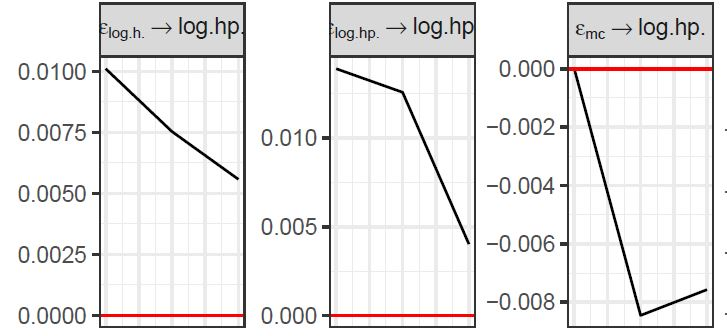
\includegraphics[width=0.9\textwidth]{hp1}
\\
Source: Own Graph
\end{figure}
\begin{figure}[H]
\label{imp2}
\caption{Impulse Response of a Shock Government Spending, Interest Rate and Output on Housing Price}
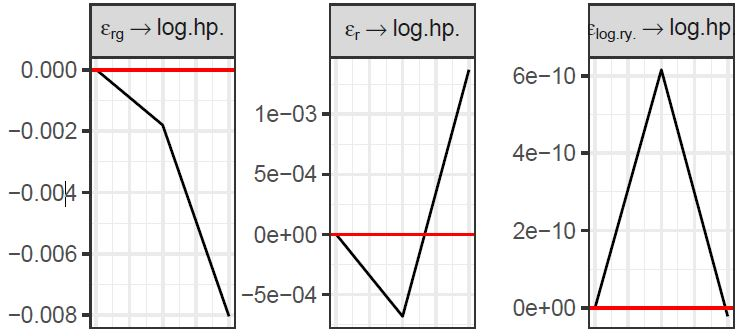
\includegraphics[width=0.9\textwidth]{hp2}
\\
Source: Own Graph
\end{figure}



\section{Conclusion}
Both models show a correlation between monetay ploicies and house price. In my opinion data is not complete for conclusion. 

%-----------------------------------
% Anhang
%-----------------------------------
\newpage
\section*{Anhang} %Überschrift "Anhang", ohne Nummerierung
\addcontentsline{toc}{section}{\langde{Anhang}\langen{Appendix}} %Den Anhang ohne Nummer zum Inhaltsverzeichnis hinzufügen
\begin{appendices}
\addtocontents{toc}{\protect\setcounter{tocdepth}{0}} %
	\renewcommand{\thesection}{\langde{Anhang}\langen{Appendix} \arabic{section}:}
	\renewcommand\thesubsection{\langde{Anhang}\langen{Appendix} \arabic{section}.\arabic{subsection}:}
	\section{Appendix}\label{Appendix}
Full Image of impulse respose is here:
\begin{figure}[H]
    \centering
    \caption[]{Beispielbild}
	\label{fig:Beispielbild}
    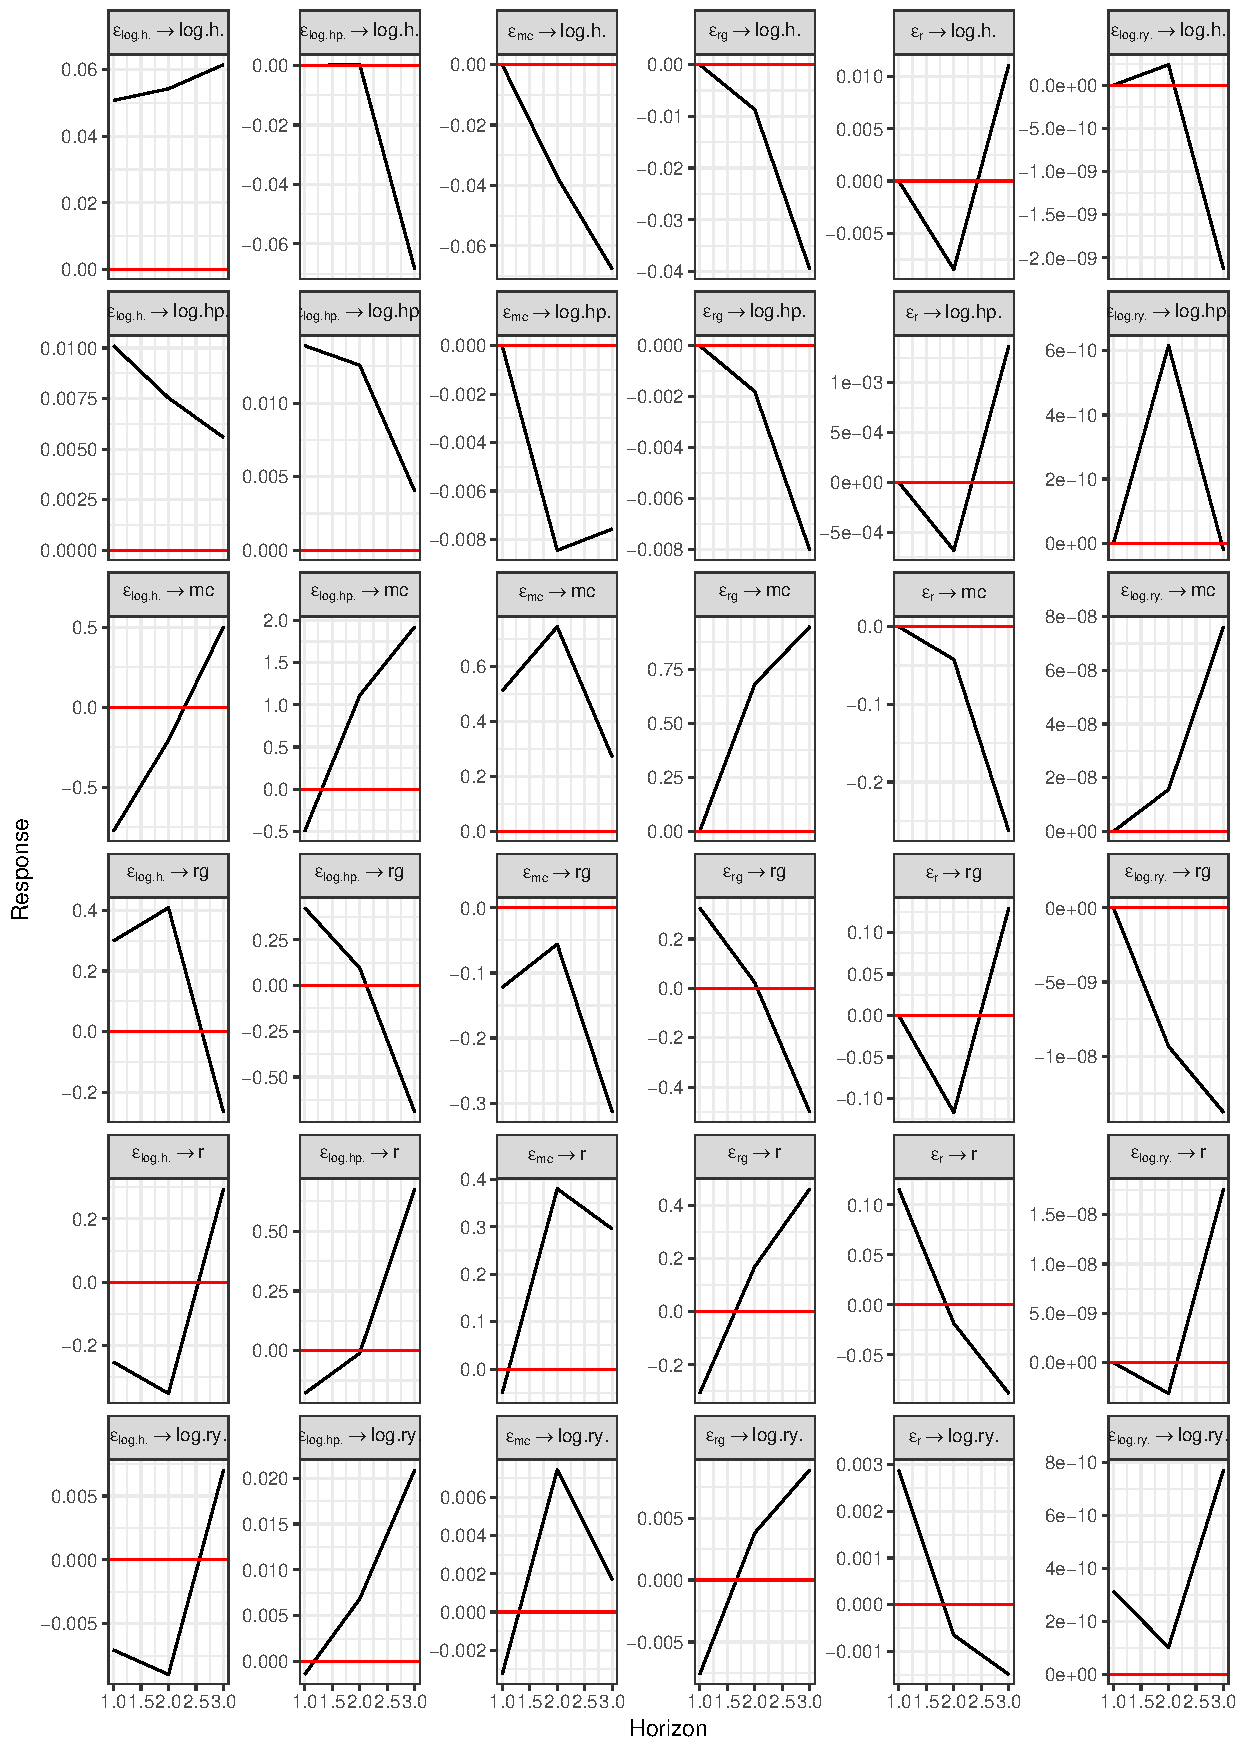
\includegraphics[width=1\textwidth]{impulseResponseTotal}
\end{figure}
\end{appendices}
\addtocontents{toc}{\protect\setcounter{tocdepth}{2}}

%-----------------------------------
% Literaturverzeichnis
%-----------------------------------
\newpage
%\addcontentsline{toc}{section}{Literatur}

% Die folgenden beiden Befehle würden ab dem Literaturverzeichnis wieder eine
% römische Seitennummerierung nutzen.
% Das ist nach dem Leitfaden nicht zu tun. Dort steht nur dass 'sämtliche
% Verzeichnisse VOR dem Textteil' römisch zu nummerieren sind. (vgl. S. 3)
%\pagenumbering{Roman} %Zähler wieder römisch ausgeben
%\setcounter{page}{4}  %Zähler manuell hochsetzen

% Ausgabe des Literaturverzeichnisses

% Keine Trennung der Werke im Literaturverzeichnis nach ihrer Art
% (Online/nicht-Online)
%\begin{RaggedRight}
%\printbibliography
%\end{RaggedRight}

% Alternative Darstellung, die laut Leitfaden genutzt werden sollte.
% Dazu die Zeilen auskommentieren und folgenden code verwenden:

% Literaturverzeichnis getrennt nach Nicht-Online-Werken und Online-Werken
% (Internetquellen).
% Die Option nottype=online nimmt alles, was kein Online-Werk ist.
% Die Option heading=bibintoc sorgt dafür, dass das Literaturverzeichnis im
% Inhaltsverzeichnis steht.
% Es ist übrigens auch möglich mehrere type- bzw. nottype-Optionen anzugeben, um
% noch weitere Arten von Zusammenfassungen eines Literaturverzeichnisse zu
% erzeugen.
% Beispiel: [type=book,type=article]
\printbibliography[nottype=online,heading=bibintoc,title={\langde{Literaturverzeichnis}\langen{Bibliography}}]

% neue Seite für Internetquellen-Verzeichnis
\newpage

% Laut Leitfaden 2018, S. 14, Fussnote 44 stehen die Internetquellen NICHT im
% Inhaltsverzeichnis, sondern gehören zum Literaturverzeichnis.
% Die Option heading=bibintoc würde die Internetquelle als eigenen Eintrag im
% Inhaltsverzeicnis anzeigen.
%\printbibliography[type=online,heading=bibintoc,title={Internetquellen}]
\printbibliography[type=online,title={\langde{Internetquellen}\langen{Internet sources}}]

%\input{kapitel/anhang/erklaerung}
\end{document}
